% 第 2 章：上同调
\chapter{上同调}\label{ch:cohomology}
本章考察若干同调与上同调理论。它们最初是在几何和拓扑的背景下发展起来的，后来则扩展到数学的许多其他领域。我们先介绍一般框架，再看拓扑和代数中的一些例子。关于这些主题的深入讨论，可参见\bookcite{111}、\bookcite{172}和\bookcite{253}。

\section{复形}\label{sec:complexes}
\takeaway{上链复形带次数为 $1$、平方为零的微分；在向量空间情形复形可分裂为 $H\oplus I\oplus R$，于是拟同构与零同伦分别归结为矩阵分量 $f^{HH}$ 是同构、为零，而 $HK^0(k)$ 等价于分次向量空间范畴。}
\subsection{定义}\label{subsec:complex-definition}
\begin{definition}{上链复形}{cochain-complex}
一个 $k$-向量空间上的上链复形\index{lianfuxing@链复形|hyperpage}\index{shanglianfuxing@上链复形|hyperpage}，是 $\mathrm{VECT}(k)$ 中对象组成的序列 $(C^i)_{i\in\mathbb Z}$，连同线性映射 $d^i\colon C^i\to C^{i+1}$，使得 $d^{i+1}d^i=0$。等价地，可以把
\[
  C^\bullet=\bigoplus_i C^i
\]
看成一个 $\mathbb Z$-分次向量空间，并在其上给定一个次数为 $1$、满足 $d^2=0$ 的线性映射 $d$。映射 $d$ 称为微分\index{weifen@微分|hyperpage}。

复形 $C^\bullet$ 的上同调\index{shangtongdiao@上同调|hyperpage}是分次向量空间
\[
  HC^\bullet:=\frac{\ker d}{\operatorname{im}d}.
\]
微分像中的元素称为恰当元，微分核中的元素称为闭元；上同调衡量闭性与恰当性之间的差别。若 $|i|$ 足够大时恒有 $C^i=0$，则称该复形有界\index{youjiefuxing@有界复形|hyperpage}。

复形 $C^\bullet$ 的 $n$ 次移位是复形 $C[n]^\bullet$，其中
\[
  C[n]^i:=C^{i+n},\qquad d_{C[n]}^i:=(-1)^n d_C^{i+n}.
\]
换言之，移位 $1$ 会使元素的次数降低 $1$，并在微分前额外引入一个负号。
% [Tutor Note: 移位同时改了两件事：指标平移 $i\mapsto i+n$，以及微分整体乘以 $(-1)^n$。后者来自把移位看作与集中在次数 $-n$ 的一维空间作张量积、再按 Koszul 规则把奇次运算符移过：每交换一次顺序就出负号，因此恰好是 $(-1)^n$。核对本章后面 $\operatorname{Hom}^\bullet(C[i],D[j])\cong\operatorname{Hom}^\bullet(C,D)[j-i]$ 所说的“适当符号”，以及第三章 $\mu_k(a_1[i_1],\ldots,a_k[i_k])$ 的移位因子时，都要从这一约定出发；漏掉 $(-1)^n$ 是最常见的移位错误。]
\end{definition}

\begin{note}
类似地，也可以考察链复形。链复形是带有次数为 $-1$ 的微分的分次向量空间 $C_\bullet$。链复形中的恰当元称为边界，闭元称为圈。

上链复形通常用上标标记次数，链复形则用下标标记。只需在指标前加负号，就可以在链复形和上链复形之间转换：
\[
  C^\bullet:=C_{-\bullet}.
\]
下文将始终使用上链复形。
\end{note}

\begin{note}
有时复形不带完整的 $\mathbb Z$-分次，而只带 $\mathbb Z_2$-分次；此时 $d$ 的次数为 $\mathbb Z_2$ 中的 $1$。这样的对象称为 $\mathbb Z_2$-复形，其同调称为 $\mathbb Z_2$-同调，我们用 $C^\pm$ 而非 $C^\bullet$ 表示它。这里采用 $\mathbb Z_2$ 的乘法记号，因此次数为 $0$ 的部分记作 $C^+$，次数为 $1$ 的部分记作 $C^-$。每个 $\mathbb Z$-复形也都是一个 $\mathbb Z_2$-复形，其中
\[
  C^+=\bigoplus_i C^{2i},\qquad C^-=\bigoplus_i C^{2i+1}.
\]
\end{note}

\begin{note}
上链复形也可以定义在任意模范畴 $\mathrm{MOD}\text{-}A$ 中，甚至可以定义在更一般的阿贝尔范畴中。阿贝尔范畴是一种线性范畴，在其中核、像和余核都有意义。
\end{note}

\subsection{态射}\label{subsec:complex-morphisms}
\begin{definition}{复形之间的态射}{complex-morphism}
上链复形 $C^\bullet,D^\bullet$ 之间的态射\index{shanglianfuxingjiandetaishe@上链复形间的态射|hyperpage}，是次数为 $0$ 的线性映射 $f\colon C^\bullet\to D^\bullet$，满足
\[
  d_Df-fd_C=0.
\]
\end{definition}
这个条件保证 $f$ 诱导出复形上同调之间的映射。事实上，若 $d_Cx=0$，则 $d_Df(x)=0$；并且 $f(d_Cy)=d_D(f(y))$。因此映射
\[
  Hf\colon HC^\bullet\longrightarrow HD^\bullet,\qquad
  x+\operatorname{im}d_C\longmapsto f(x)+\operatorname{im}d_D
\]
是良定义的，并且与复合相容：$H(f\circ g)=Hf\circ Hg$。

\begin{definition}{拟同构与同伦}{quasi-isomorphism}
复形态射 $f\colon C^\bullet\to D^\bullet$ 称为
\begin{enumerate}
  \item 拟同构\index{nitonggou@拟同构|hyperpage}，若 $Hf$ 是同构；
  \item 零同伦\index{lingtonglun@零同伦|hyperpage}，若存在一个次数为 $-1$ 的线性映射 $g\colon C^\bullet\to D^\bullet$，使得
  \[
    f=d_Dg+gd_C.
  \]
  在这种情况下 $Hf=0$。
\end{enumerate}
若两个态射之差是零同伦的，则称这两个态射彼此同伦\index{tongluntaishe@同伦态射|hyperpage}。
\end{definition}

给定两个复形 $C^\bullet,D^\bullet$，可以构造由任意次数的分次模态射组成的复形 $\operatorname{Hom}^\bullet(C^\bullet,D^\bullet)$：
\[
  \operatorname{Hom}^j(C^\bullet,D^\bullet)
  :=\bigoplus_i\operatorname{Hom}_k(C^i,D^{i+j}),\qquad
  df=d_Df-(-1)^{\deg f}fd_C.
\]
这仍是一个上链复形，因为其微分次数为 $+1$。这个复形的零次上同调给出模去链同伦后的复形态射，也就是链同伦类。其他次数的上同调也可以解释为移位复形之间的态射，因为
\[
  \operatorname{Hom}^\bullet(C[i]^\bullet,D[j]^\bullet)
  \cong\operatorname{Hom}^\bullet(C^\bullet,D^\bullet)[j-i],
\]
其中的同构还会按适当方式加入符号。

\subsection{复形的结构定理}\label{subsec:complex-structure}
\begin{definition}{极小复形与可缩复形}{minimal-contractible}
设 $C^\bullet$ 是一个上链复形。
\begin{enumerate}
  \item 若其微分为零，则称 $C^\bullet$ 为极小复形\index{jixiaofuxing@极小复形|hyperpage}；
  \item 若其同调为零，则称 $C^\bullet$ 为可缩复形\index{kesuofuxing@可缩复形|hyperpage}。
\end{enumerate}
\end{definition}
若给复形的同调赋予零微分，就可以把它看作一个极小复形。这个想法导出下面的结构定理。

\begin{theorem}{复形的分解}{complex-decomposition}
每个 $k$-向量空间复形 $C^\bullet$ 都是一个可缩复形与一个极小复形的直和。
\end{theorem}
\begin{proof}[证明思路]
由于 $C^i$ 是向量空间，我们可以选取直和分解
\[
  C^i=H^i(C)\oplus I^i(C)\oplus R^i(C),
\]
使得
\[
  \operatorname{im}d=I^\bullet(C),\qquad
  \ker d=H^\bullet(C)\oplus I^\bullet(C),
\]
并且 $d\colon R^i(C)\to I^{i+1}(C)$ 是同构。注意，$C_m^\bullet:=H^\bullet(C)$ 和 $C_c^\bullet:=I^\bullet(C)\oplus R^\bullet(C)$ 都是 $C^\bullet$ 的子复形。前者是极小复形，后者是可缩复形。
\end{proof}
% [Tutor Note: 证明第一步“由于 $C^i$ 是向量空间”是关键：它保证了每个子空间都有直和补，才能把 $C^i$ 拆成 $H\oplus I\oplus R$ 并使 $d\colon R^i\to I^{i+1}$ 同构。换成 $\mathbb Z$-模（例如 $\mathbb Z\xrightarrow{2}\mathbb Z$）这一步就失效，结构定理与后面的拟同构判别引理都不再成立，见练习 2.1。一般的阿贝尔范畴里同样没有这种分裂。]
上述分解使每个线性映射 $\varphi\colon C^\bullet\to D^\bullet$ 都能分解成九个分量，例如 $\varphi^{IH}\colon H^\bullet(C)\to I^\bullet(D)$ 等。

\begin{lemma}{拟同构与同伦的判别}{complex-map-criterion}
设 $f\colon C^\bullet\to D^\bullet$ 是 $k$-向量空间上链复形之间的态射。
\begin{enumerate}
  \item $f$ 是拟同构，当且仅当 $f^{HH}$ 是同构；
  \item $f$ 零同伦，当且仅当 $f^{HH}=0$；
  \item 映射
  \[
    \pi\colon H\operatorname{Hom}^\bullet(C^\bullet,D^\bullet)
    \longrightarrow\operatorname{Hom}^\bullet(HC^\bullet,HD^\bullet),
    \qquad f\longmapsto\bar f=f^{HH}
  \]
  是同构；
  \item 复形态射 $f\colon C^\bullet\to D^\bullet$ 是拟同构，当且仅当存在态射 $f^\dagger\colon D^\bullet\to C^\bullet$，使得 $f^\dagger f$ 与 $ff^\dagger$ 分别同伦于 $1_C$ 和 $1_D$。这样的 $f^\dagger$ 称为 $f$ 的拟逆\index{nini@拟逆|hyperpage}。
\end{enumerate}
\end{lemma}
\begin{proof}[证明思路]
第一条显然成立，因为按构造，$H^\bullet(-)$ 与复形的同调自然等同。证明第二条时注意，根据上述分解，微分具有如下矩阵形式：
\[
  d=\begin{pmatrix}0&0&\delta\\0&0&0\\0&0&0\end{pmatrix},
\]
其中 $\delta$ 可逆。

\begin{figure}[H]\centering
  \centering
  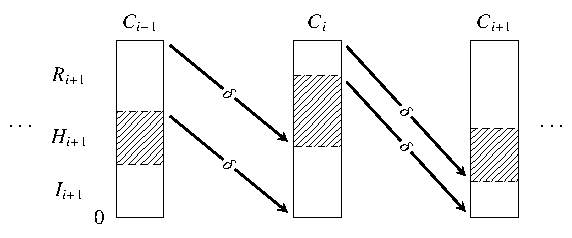
\includegraphics[width=0.54\paperwidth]{figures/Fig_001_PDF030_Book018.pdf}
  \caption{复形分解中的 $H$、$I$、$R$ 分量及微分（原书 p.18）}
  \label{fig:complex-splitting}
\end{figure}

令
\[
  h=\begin{pmatrix}0&0&0\\0&0&0\\\delta^{-1}&0&0\end{pmatrix}.
\]
容易验证，$dh$、$hd$ 和 $1-dh-hd$ 是分别投影到三个分量上的幂等元 $e_I,e_R,e_H$。此外还有
\[
  h^2=0,\qquad dhd=d,\qquad hdh=h.
\]
若 $f$ 是复形态射且 $f^{HH}=0$，则
\begin{align*}
  0=f^{HH}=e_Hfe_H
   &=f-dhf-hdf-fdh+dhfdh+hdfdh-fhd+dhfhd+hdfhd\\
   &=f-dhf-hdf-dfh+dfh+0-fhd+dhfhd+hfd\\
   &=f-dhf-fhd+dhfhd\\
   &=f-\bigl(d(hf-dhfh)+(hf-dhfh)d\bigr).
\end{align*}
因此 $f=dg+gd$，其中 $g=hf-dhfh$，所以 $f$ 零同伦。

第三条中，$\pi$ 的单射性直接由第二条得到；任意仅有 $f^{HH}$ 分量非零的映射都是复形态射，故 $\pi$ 也是满射。证明第四条时，取 $f^\dagger$ 为 $(f^{HH})^{-1}$ 在 $\pi$ 下的任意原像即可。
\end{proof}
% [Tutor Note: 这里出现的 $h^2=0$、$dhd=d$、$hdh=h$ 不是随手选出的恒等式，而是“收缩数据”的典型关系（还配上 $dh$、$hd$ 为投影、$h$ 次数为 $-1$）。第三章的同调扰动引理正是把这组关系抽象为 $\varphi\varphi^\dagger=1_B+h\mu_1^B+\mu_1^Bh$ 等条件，再据此把 $A_\infty$ 结构沿 $h$ 搬运过去；记住这套关系，后面的树形公式才看得懂。]

\subsection{范畴观点}\label{subsec:complex-category}
从更抽象的角度看，可以引入范畴 $K^\bullet(k)$。它的对象是 $k$-向量空间上的上链复形，态射为所有 $k$-线性映射：
\[
  K^\bullet(k)(C^\bullet,D^\bullet)
  =\operatorname{Hom}^\bullet(C^\bullet,D^\bullet).
\]
这个范畴实际上是微分分次范畴（简称 dg-范畴\index{dgfanchou@dg-范畴|hyperpage}）。这是一类特殊的 $k$-线性范畴，其 Hom 空间本身是上链复形，且微分满足分次 Leibniz 律：
\[
  d(f\circ g)=df\circ g+(-1)^{\deg f}f\circ dg.
\]

若要在拟同构意义下研究复形，就必须转到拟同构可逆的范畴。这可以通过考察 $HK^0(k)$ 来实现：其对象仍是 $k$-向量空间复形，Hom 空间则为 $H\operatorname{Hom}^0(C^\bullet,D^\bullet)$。由引理\ref{lem:complex-map-criterion}，这个范畴等价于分次 $k$-向量空间范畴 $\mathrm{grVECT}(k)$，其中态射是次数为 $0$ 的齐次线性映射。具体而言，函子
\[
  \pi\colon HK^0(k)\longrightarrow\mathrm{grVECT}(k),\qquad
  C^\bullet\longmapsto HC^\bullet,\quad
  f\longmapsto Hf\cong f^{HH}
\]
是范畴等价。

\begin{note}
前两节的讨论针对向量空间复形。若向量空间还带有额外结构，例如环结构或 $k$-代数 $A$ 上的模结构，这些结构通常不会在上述分解中保留下来，我们构造的拟逆也未必与额外结构相容。因此，当 $A$ 是代数时，需要调整 $HK^0(A)$ 的构造。第三章将详细讨论这一点。
\end{note}

\section{拓扑中的上同调}\label{sec:topology-cohomology}
\takeaway{$\Delta$-集是函子 $\Delta^{\mathrm{op}}\to\mathrm{Sets}$，其单纯上链复形带杯积，因而有上同调环；实现同一拓扑空间的 $\Delta$-集给出同构的上同调环（拓扑不变性），德拉姆上同调经积分映射与之拟同构；Massey 积作为高阶运算可以区分环结构区分不了的博罗米恩环。}
\subsection{粘合单形}\label{subsec:gluing-simplices}
许多拓扑空间（例如多面体）都可以由较小的部分粘合而成。若要描述一个由三角形构成的多面体，我们需要给出一组三角形、一组边和一组点；此外，还要给每个三角形指定三条边，并给每条边指定两个端点。利用 $\Delta$-集\index{deltaji@$\Delta$-集|hyperpage}，可以简洁地描述这些数据\bookcite{209}。\footnote{文献中也称之为 $\Delta$-复形\bookcite{111}。我们更愿称其为 $\Delta$-集，因为“复形”一词在本书中用于上链复形。$\Delta$-集与更常见的单纯集概念密切相关\bookcite{87}。}

\begin{definition}{严格单调递增单形范畴}{simplex-category}
严格单调递增单形范畴\index{yangedandiaodizengdanxingfanchou@严格单调递增单形范畴|hyperpage} $\Delta$ 的对象是所有集合
\[
  [n]:=\{0,\ldots,n\},\qquad n\geq 0,
\]
其态射是所有严格递增映射：
\[
  \Delta([m],[n])
  =\{\varphi\colon[m]\to[n]\mid x>y\Longrightarrow\varphi(x)>\varphi(y)\}.
\]
所有严格递增映射都是单射，并且可以由一些特殊映射——面映射\index{mianyingshe@面映射|hyperpage}——复合而成。面映射是把 $[n-1]$ 映入 $[n]$ 并跳过一个元素的单射：
\[
  \delta_i\colon[n-1]\to[n],\qquad
  x\longmapsto
  \begin{cases}
    x,&x<i,\\
    x+1,&x\geq i.
  \end{cases}
\]
\end{definition}

我们还可以用几何方式实现这个范畴。标准 $n$-单形是拓扑空间
\[
  \operatorname{Simp}_n
  :=\left\{(x_0,\ldots,x_n)\in[0,1]^{n+1}\ \middle|\ \sum_{i=0}^n x_i=1\right\}.
\]
因此 $\operatorname{Simp}_0$ 是一个点，$\operatorname{Simp}_1$ 是线段，$\operatorname{Simp}_2$ 是三角形，依此类推。
\begin{figure}[H]\centering
  \centering
  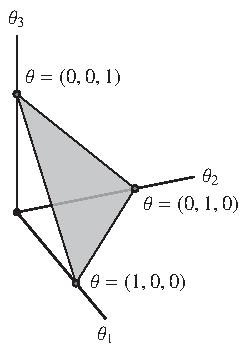
\includegraphics[width=0.46\paperwidth]{figures/Fig_002_PDF032_Book020.pdf}
  \caption{标准单形 $\operatorname{Simp}_2$ 及其顶点坐标（原书 p.20）}
  \label{fig:standard-simplex}
\end{figure}
面映射可以实现为各个面的嵌入（标准单形及其顶点坐标见图\ref{fig:standard-simplex}）：
\[
  \delta_i\colon\operatorname{Simp}_{n-1}\to\operatorname{Simp}_n,\qquad
  (x_0,\ldots,x_{n-1})\longmapsto
  (x_0,\ldots,x_{i-1},0,x_i,\ldots,x_{n-1}).
\]
几何严格单形范畴的对象是标准单形，态射由面映射生成。按构造，它与 $\Delta$ 等价。

设某个拓扑空间由点、线段、三角形等拼成，并且每个这样的对象都与一个标准 $n$-单形相对应。对于每个 $n$-单形，我们可以给出与之对应的对象所成的集合。若有映射 $\varphi\colon\operatorname{Simp}_n\to\operatorname{Simp}_m$，并且某个对象与标准 $m$-单形相对应，那么将 $\varphi$ 与这个对应复合，就会得到一个把标准 $n$-单形对应到另一个对象的映射。因此，$\varphi$ 给出从与 $m$-单形对应的对象到与 $n$-单形对应的对象的映射。这引出以下定义。

\begin{definition}{$\Delta$-集}{delta-set}
$\Delta$-集是反变函子 $S\colon\Delta\to\mathrm{Sets}$。与 $\Delta$-集相联系的几何实现\index{jiheshixian@几何实现|hyperpage}为
\[
  |S|:=\left(\coprod_i S[i]\times\operatorname{Simp}_i\right)\big/\sim,
\]
其中对每个态射 $\varphi\in\Delta$，规定
\[
  (a,\varphi(x))\sim(S(\varphi)(a),x).
\]
\end{definition}
注意，若 $\varphi$ 是面映射 $\delta_i$，上述等价关系便意味着：与 $a$ 的第 $i$ 个面对应的单形（即形如 $(S(\delta_i)(a),x)$ 的点）会与 $a$ 所对应单形中该面的嵌入（即形如 $(a,\delta_i(x))$ 的点）粘合。

\begin{example}[环面与球面的 $\Delta$-集]\label{ex:torus-sphere-delta}
\begin{enumerate}
  \item 环面 $S^1\times S^1$ 可以由函子 $S$ 实现，其中
  \[
    S[0]=\{P\},\qquad S[1]=\{\ell_0,\ell_1,\ell_2\},\qquad S[2]=\{a,b\}.
  \]
  面映射的作用为 $S(\delta_i)(\ell_j)=P$、$S(\delta_i)(a)=\ell_i$、$S(\delta_i)(b)=\ell_{2-i}$。
  \item 球面 $S^2$ 可以由函子 $S$ 实现，其中
  \[
    S[0]=\{p,q,r\},\qquad S[1]=\{\ell_0,\ell_1,\ell_2\},\qquad S[2]=\{a,b\}.
  \]
  面映射的作用满足 $S(\delta_i)(a)=\ell_i$、$S(\delta_i)(b)=\ell_i$；而对边 $\ell_j$，当 $i=1$ 时 $S(\delta_i)(\ell_j)$ 是其头端点，当 $i=0$ 时是其尾端点（见图\ref{fig:torus-sphere-delta}）。
\end{enumerate}
\end{example}
\begin{figure}[H]\centering
  \centering
  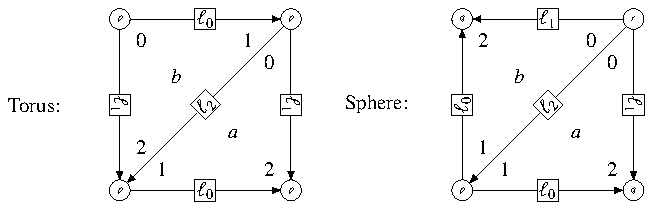
\includegraphics[width=0.82\textwidth]{figures/Fig_003_PDF033_Book021.pdf}
  \caption{环面与球面的 $\Delta$-集实现（原书 p.21）}
  \label{fig:torus-sphere-delta}
\end{figure}
不同的 $\Delta$-集可能给出同胚的拓扑空间。为了对此加以控制，我们希望定义只依赖于拓扑实现的拓扑不变量。

\subsection{单纯上同调}\label{subsec:simplicial-cohomology}
\begin{definition}{$\Delta$-集的单纯上同调}{simplicial-cohomology}
设 $S$ 是一个 $\Delta$-集，$k$ 是一个域。定义向量空间上链复形
\[
  C_\Delta^i(S,k):=\mathrm{Sets}(S[i],k),
\]
其微分为
\[
  df=\sum_j(-1)^j f\circ\delta_j.
\]
容易验证 $d^2=0$。复形 $C_\Delta^\bullet(S,k)$ 的上同调称为 $S$ 的单纯上同调\index{danchunshangtongdiao@单纯上同调|hyperpage}，记为 $H^\bullet(S,k)$。
\end{definition}

\begin{note}
这一构造可以分成两步：
\begin{enumerate}
  \item 将 $S$ 与函子 $\mathrm{Sets}(-,k)$ 复合，把它变成左 $\Delta$-模 $M\colon\Delta\to\mathrm{VECT}(k)$；
  \item 将左 $\Delta$-模 $M$ 变成上链复形 $M^\bullet$，其中 $M^i=M[i]$，且 $d=\sum_j(-1)^jM(\delta_j)$。
\end{enumerate}
在某些情形下，$\Delta$-集本身已经带有 $\Delta$-模结构，此时可以略去第一步。
\end{note}

如何理解单纯上链复形？注意，$f\in C_\Delta^i(S,k)$ 把每个 $i$-单形对应到一个数，可以把它想成流经该单形的流量。从这个角度看，$df$ 衡量流经每个 $(i+1)$-单形边界的流入与流出之差。若 $df=0$，则流量不会在某个 $(i+1)$-单形中累积，因此它表示一个闭流。若 $\Delta$-集有一个洞（例如缺少某个 $(i+1)$-单形），闭流就可能在那个缺失的单形处累积。这类流却不会是恰当的，因而会在上同调中留下非零类。因此，可以说 $S$ 的上同调测量了拓扑空间 $|S|$ 中的洞。
\begin{figure}[H]\centering
  \centering
  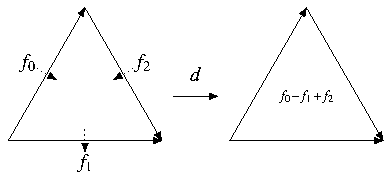
\includegraphics[width=0.48\paperwidth]{figures/Fig_004_PDF034_Book022.pdf}
  \caption{单纯上链中的流量与边界微分（原书 p.22）}
  \label{fig:cochain-flow}
\end{figure}

\begin{definition}{杯积}{cup-product}
上链复形 $C_\Delta^\bullet(S,k)$ 带有自然乘积。若 $f\in C_\Delta^p(S,k)$、$g\in C_\Delta^q(S,k)$，定义杯积\index{beiji@杯积|hyperpage} $f\smile g\in C_\Delta^{p+q}(S,k)$ 为
\[
  (f\smile g)(a):=f(S(\iota_p)(a))\cdot g(S(\upsilon_q)(a)),
\]
其中 $\iota_p$ 是包含映射 $[p]=\{0,\ldots,p\}\subset\{0,\ldots,p+q\}=[p+q]$，而
\[
  \upsilon_q\colon[q]\to[p+q],\qquad x\longmapsto x+p.
\]
可以验证，这个乘积满足结合律和分次 Leibniz 律：
\[
  d(f\smile g)=df\smile g+(-1)^p f\smile dg.
\]
因此，上同调上也定义了乘积：若 $df=dg=0$，则 $d(f\smile g)=0$，所以闭元的乘积仍是闭元。此外，
\[
  (f+dh)\smile g=f\smile g+d(h\smile g),
\]
因此给 $f$ 加上恰当元不会改变乘积的上同调类。
% [Tutor Note: 原书此处把末式印成 $(f+dh)\smile g=f\smile g-d(h\smile g)$，符号有误：由 $d(h\smile g)=dh\smile g+(-1)^{|h|}h\smile dg$ 与 $dg=0$ 得 $d(h\smile g)=dh\smile g$，故应为加号（译文已按加号排）。另外注意两处符号的不同来源：Leibniz 律里的 $(-1)^p$ 来自 $f$ 的次数 $p$，而末式的成立只用 $dg=0$，$df=0$ 仅用于保证 $[f]$ 是上同调类。]
\end{definition}

\begin{definition}{上同调环}{cohomology-ring}
配备杯积的空间 $HC_\Delta^\bullet(S,k)$ 称为 $S$（系数取 $k$）的上同调环\index{shangtongdiaohuan@上同调环|hyperpage}，记作 $H^\bullet(S,k)$。
\end{definition}

\begin{example}[环面的上同调环]\label{ex:torus-cohomology-ring}
利用例\ref{ex:torus-sphere-delta}中的 $\Delta$-集计算环面的上同调环。令 $P$ 表示在所有顶点上取 $1$ 的常函数；$L_0,L_1,L_2,A,B$ 分别表示在 $\ell_0,\ell_1,\ell_2,a,b$ 上取 $1$、在其余顶点上取 $0$ 的函数。微分满足
\[
  dP=dA=dB=0,\qquad dL_i=(-1)^{i+1}(A+B),
\]
因此上同调的一组基为 $[P]$、$[L_0+L_1]$、$[L_2+L_1]$ 和 $[A]=-[B]$。所有单形的角点都是 $p$，故 $P\smile X=X$。此外，对 $a$ 有 $S(\iota_1)(a)=\ell_2$、$S(\upsilon_1)(a)=\ell_0$；对 $b$ 则相反，即 $S(\iota_1)(b)=\ell_0$、$S(\upsilon_1)(b)=\ell_2$。因此
\[
  L_0\smile L_2=B,\qquad L_2\smile L_0=A,
\]
而 $L_i$ 之间的其他乘积均为零。由此得到上同调环
\[
  HC_\Delta^\bullet(S,k)\cong
  \frac{k\langle\xi,\eta\rangle}{\langle\xi\eta+\eta\xi,\xi^2,\eta^2\rangle},
\]
其中
\[
  1=[P],\qquad \xi=[L_0+L_1],\qquad
  \eta=[L_2+L_1],\qquad
  \xi\eta=[B]=-[A]=-\eta\xi.
\]
\end{example}

几何实现同胚的不同 $\Delta$-集会给出不同的上链复形，但其上同调环相同。证明这一点的一种方法，是把它们与只依赖空间 $X=|S_1|=|S_2|$ 的上同调环联系起来。

\begin{definition}{奇异上同调环}{singular-cohomology}
对拓扑空间 $X$，定义 $\Delta$-集 $X$，其 $i$-单形是从 $\operatorname{Simp}_i$ 到 $X$ 的所有连续映射：
\[
  X[i]=\mathrm{Top}(\operatorname{Simp}_i,X),\qquad
  X[\delta_i](f)=f\circ\delta_i.
\]
上同调环 $HC_\Delta^\bullet(X,k)$ 称为 $X$ 的奇异上同调环\index{qiyishangtongdiaohuan@奇异上同调环|hyperpage}，记作
\[
  H^\bullet(X,k):=HC_\Delta^\bullet(X,k).
\]
\end{definition}

\begin{theorem}{拓扑不变性}{topological-invariance}
若 $S$ 是一个几何实现为 $X=|S|$ 的 $\Delta$-集，则
\[
  HC_\Delta^\bullet(S,k)\cong H^\bullet(X,k)
\]
作为分次环同构。
\end{theorem}
\begin{proof}[证明思路]
单纯复形 $S$ 自然嵌入到 $X$ 中，从而给出一个限制映射
\[
  C_\Delta^\bullet(X,k)\longrightarrow C_\Delta^\bullet(S,k),
\]
它是 dg-代数态射。可以证明该映射是拟同构，因此在上同调层面诱导出分次环同构。更多信息见\bookcite{111}。
\end{proof}

\begin{note}
设两个 $\Delta$-集 $S_1,S_2$ 满足 $|S_1|\cong|S_2|=X$，则有如下图式，其中两条实线箭头是环的拟同构：
\begin{figure}[H]\centering
  \centering
  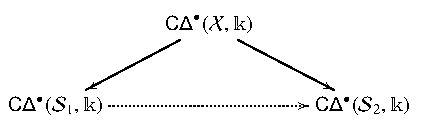
\includegraphics[width=0.43\paperwidth]{figures/Fig_005_PDF036_Book024.pdf}
  \caption{由同一拓扑空间诱导的上链复形之间的拟同构（原书 p.24）}
  \label{fig:topological-quasi-isomorphisms}
\end{figure}
由引理\ref{lem:complex-map-criterion}，存在一个使图交换的向量空间拟同构：将第二个投影与第一个投影的拟逆复合即可。遗憾的是，这个拟同构一般不是环的拟同构。
\end{note}

\subsection{德拉姆上同调}\label{subsec:de-rham-cohomology}
设 $M$ 是光滑、紧致、可定向流形。回忆一下，$k$-形式是反对称积 $\Lambda^kT^*M$ 的一个截面。在局部坐标中，可以写成
\[
  \omega=\sum_{i_1<\cdots<i_k}
  \omega_{i_1\ldots i_k}\,dx_{i_1}\wedge\cdots\wedge dx_{i_k},
\]
其微分为
\[
  d\omega=
  \sum_{i_1<\cdots<i_k}\sum_j
  \frac{\partial\omega_{i_1\ldots i_k}}{\partial x_j}
  \,dx_j\wedge dx_{i_1}\wedge\cdots\wedge dx_{i_k},
\]
这里采用约定 $dx_i\wedge dx_j=-dx_j\wedge dx_i$。$k$-形式空间记作 $\Omega^k(M)$。

\begin{definition}{德拉姆复形与德拉姆上同调}{de-rham-complex}
三元组 $(\Omega^\bullet(M),d,\wedge)$ 构成一个 dg-代数，称为德拉姆复形\index{delamufuxing@德拉姆复形|hyperpage}。这个复形的上同调环称为德拉姆上同调\index{delamushangtongdiao@德拉姆上同调|hyperpage}：
\[
  H_{\mathrm{dR}}^\bullet(M):=H\Omega^\bullet(M).
\]
\end{definition}
若 $f\colon\operatorname{Simp}_k\to M$ 是光滑映射，则可以拉回任意 $k$-形式 $\omega\in\Omega^k(M)$ 并对其积分。若 $S$ 是满足 $|S|\cong M$ 的 $\Delta$-集，这一过程给出映射
\[
  \varphi\colon\Omega^\bullet(M)\longrightarrow C_\Delta^\bullet(S,\mathbb R),
  \qquad \omega\longmapsto\bigl(a\longmapsto\int_a\omega\bigr),
\]
其中 $\int_a$ 表示在 $|S|\cong M$ 中嵌入的单形 $\{a\}\times\operatorname{Simp}_k$ 上积分。斯托克斯定理表明该映射是复形态射：
\[
  \varphi(d\omega)(a)=\int_a d\omega
  =\int_{\partial a}\omega
  =\sum_i\pm\int_{\delta_i a}\omega
  =d\varphi(\omega)(a).
\]
该映射还与乘积相容，因此有如下定理。其证明和更多细节可参见\bookcite{45}。

\begin{theorem}{德拉姆定理}{de-rham-theorem}
映射 $\varphi\colon\Omega^\bullet(M)\to C_\Delta^\bullet(S,\mathbb R)$ 是拟同构。
\end{theorem}

\subsection{Massey 积}\label{subsec:massey-products}
从 $C_\Delta^\bullet(S,\mathbb R)$ 或 $\Omega^\bullet(M)$ 上的乘积过渡到上同调上的乘积，往往会损失信息。为弥补这一点，可以引入称为 Massey 积\index{masseyji@Massey 积|hyperpage}的高阶乘积。Massey 积是一种构造新上同调类的方法：给定一列满足某些附加条件的上同调类，可以由它们得到新的上同调类。

三元 Massey 积的构造如下。取三个上同调类 $[u],[v],[w]$，并假设 $[u\smile v]=[v\smile w]=0$。这意味着存在元素 $s,t\in C_\Delta^\bullet(S,k)$，使得
\[
  u\smile v=ds,\qquad v\smile w=dt.
\]
利用 Leibniz 律可得
\[
  d(u\smile t)=du\smile t\pm u\smile dt=\pm u\smile v\smile w,
\]
\[
  d(s\smile w)=ds\smile w\pm s\smile dw=u\smile v\smile w.
\]
因此，选取适当的符号后，有 $d(u\smile t\pm s\smile w)=0$，于是可以考察上同调类 $[u\smile t\pm s\smile w]$。注意其定义取决于 $s,t$ 的选择；Massey 积 $\langle[u],[v],[w]\rangle$ 定义为改变 $s,t$ 后所有可能得到的上同调类所成的集合。
% [Tutor Note: 三个要点：其一，$\langle[u],[v],[w]\rangle$ 一般是一个集合而非单个类（只有当它只含一个元素时才说“良定义”），所以博罗米恩环那个例子的结论写成“含有非零类/只含零类”。其二，两处的 $\pm$ 必须取相容的符号，最终类才闭；不同 $s,t$ 给出的类相差 $\pm$ 恰当项。其三，这一“选 $s,t$ 再取类”的不定性，正是第三章 $A_\infty$ 语言中 $\mu_3$ 只定义到同伦（或到 $\pm$）的原因。]

\begin{example}[博罗米恩环与 Massey 积]\label{ex:borromean-massey}
设 $S$ 是一个实现单位立方体 $[0,1]^3$ 的 $\Delta$-集。令 $\gamma_1,\gamma_2,\gamma_3\colon S^1\to(0,1)^3$ 是嵌入单位立方体的三条两两不交的圆周，并假设每个单形至多与其中一条曲线相交，且交集只是一段区间。定义 $S_\gamma$ 为由所有与 $\gamma_i$ 不相交的单形构成的 $\Delta$-集。

固定单位立方体中以 $\gamma_i$ 为边界的圆盘 $D_i$，并定义 $\lambda_i\in H^1(S_\gamma,k)$ 如下：
\[
  \text{对每个 }a\in S[1],\qquad
  \lambda_i(a)=
  \begin{cases}
    1,&a\text{ 沿正向穿过 }D_i,\\
    -1,&a\text{ 沿负向穿过 }D_i,\\
    0,&a\text{ 不穿过 }D_i.
  \end{cases}
\]
虽然这个定义依赖于 $D_i$ 的选择，但其上同调类只依赖于 $\gamma_i$。

若 $\gamma_i$ 与 $\gamma_j$ 互不链接，则可以证明 $\lambda_i\smile\lambda_j=0\in H^2(S_\gamma,k)$；若它们像霍普夫链环那样相互套链，则 $\lambda_i\smile\lambda_j\neq0$。
\begin{figure}[H]\centering
  \centering
  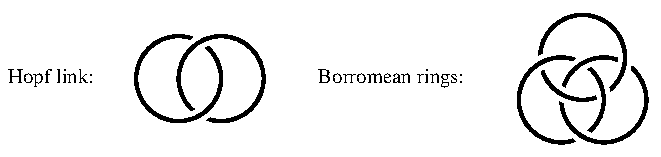
\includegraphics[width=0.62\paperwidth]{figures/Fig_006_PDF038_Book026.pdf}
  \caption{霍普夫链环与博罗米恩环（原书 p.26）}
  \label{fig:hopf-borromean}
\end{figure}
博罗米恩环是嵌入三维空间中的三条环：忽略其中任意一条，另外两条都可以在不相交的情况下分开；但三条环整体却不能分开。因此，对所有 $i,j$，都有 $\lambda_i\smile\lambda_j=0$，这正是可以定义 Massey 积的情形。Massey 在\bookcite{171}中计算得出，$\langle\lambda_1,\lambda_2,\lambda_3\rangle$ 含有一个非零上同调类；而对三条完全没有相互链接的圆周进行同样计算时，$\langle\lambda_1,\lambda_2,\lambda_3\rangle$ 只含零类。
\end{example}

上同调环的环结构无法区分博罗米恩环与彼此松散的三条环，但 Massey 积可以。在下一章中，我们将看到一种增强上同调环的方式，把这些高阶乘积也纳入其中。

\section{代数中的上同调}\label{sec:algebra-cohomology}
把复杂空间切分为较简单的部分并研究它们如何粘合起来，这一思想可以推广到数学的许多领域。本节将在代数的表示论中考察这一思路。

\takeaway{自由分解把模的问题化为自由模复形的计算：比较定理保证提升存在且在同伦意义下唯一，故 $\operatorname{Ext}$ 群与 Ext 环不依赖分解的选择；Koszul 分解把 $\operatorname{Ext}^\bullet_A(S,S)$ 算成与生成元、关系对偶的代数，而乘法只能恢复关系的二次部分。}

\subsection{分解}\label{subsec:resolutions}
设 $A$ 是 $k$ 上的代数，$M$ 是右 $A$-模。若 $M$ 由集合 $S^0$ 生成，就可以从自由模构造一个到 $M$ 的满射：
\[
  M\longleftarrow\bigoplus_{m\in S^0}A=:P^0.
\]
这个映射的核有一个生成集 $S^1$，因而可以构造映射
\[
  P^0\longleftarrow\bigoplus_{m\in S^1}A=:P^{-1}.
\]
如此继续下去（并令 $i>0$ 时 $P^i=0$），最终得到一个由自由模构成的上链复形 $P^\bullet$。按构造，该复形的同调在次数 $0$ 等于 $M$，其他次数均为零。

\begin{definition}{自由分解}{free-resolution}
右 $A$-模 $M$ 的自由分解\index{ziyoufenjie@自由分解|hyperpage}，是一个由自由 $A$-模构成的复形 $P^\bullet$，满足 $HP^\bullet=M^\bullet$；这里 $M^\bullet$ 表示仅在次数 $0$ 有 $M$、其他次数均为零的复形。
\end{definition}
注意，这一构造并不能给出唯一的自由分解，因为它取决于生成元的选择。不过可以证明，$M$ 的任意两个自由分解都拟同构。进一步还有以下引理。

\begin{theorem}{比较定理}{comparison-theorem}
若 $\varphi\colon M\to N$ 是态射，且 $P^\bullet,Q^\bullet$ 分别是 $M,N$ 的自由分解，则存在复形态射 $\bar\varphi$，使其在同调上诱导的态射为 $\varphi$。这个提升在相差同伦的意义下唯一。
\end{theorem}
\begin{proof}[证明思路]
思路是逐步构造 $\bar\varphi$：因为 $Q^0\to N$ 是满射，可以找到 $q_i\in Q^0$，使它们分别映到 $P^0\to M\to N$ 下各生成元的像。将 $P^0$ 的生成元映到这些 $q_i$，就得到 $P^0$ 上的提升 $\bar\varphi^0$。
\begin{figure}[H]\centering
  \centering
  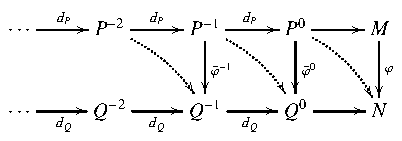
\includegraphics[width=0.52\paperwidth]{figures/Fig_007_PDF040_Book028.pdf}
  \caption{自由分解之间对模态射的逐步提升（原书 p.28）}
  \label{fig:comparison-theorem-lift}
\end{figure}
现在考察 $P^{-1}$ 的生成元经 $\bar\varphi^0d_P$ 后的像。由提升性质，这些像落在 $Q^0\to N$ 的核中，因此可以找到它们在 $d_Q$ 下的原像。把 $P^{-1}$ 的生成元映到这些原像，就得到 $\bar\varphi^{-1}$。随后考察 $P^{-2}$ 的生成元，并重复同一过程，最终构造出整个 $\bar\varphi$。唯一性可用类似论证证明；见\bookcite[定理 2.2.6]{253}。
\end{proof}
% [Tutor Note: “唯一性可用类似论证证明”省掉的正是同伦 $s$ 的构造，其归纳步骤是：在次数 $0$，差 $\bar\psi^0-\bar\varphi^0$ 是闭的且落在 $\ker(Q^0\to N)=\operatorname{im}d_Q$ 中，用 $P^0$ 的自由性提升得到 $s^0$ 使 $\bar\psi^0-\bar\varphi^0=d_Qs^0$；随后考察 $\bar\psi^{i}-\bar\varphi^{i}-s^{i-1}d_P$（$i<0$），它仍是闭的且落在 $\operatorname{im}d_Q$ 中，再提升一次。每一步都依赖 $P^\bullet$ 由自由（或投射）模构成，这就是定理必须对这类分解陈述的原因。]
特别地，对 $\varphi$ 取恒等态射 $1_M$，便得到 $M$ 的任意一对自由分解 $P^\bullet,Q^\bullet$ 之间的拟同构。

\begin{note}
除了自由分解，也可以使用更一般的投射分解，其中每个分量都是投射 $A$-模（即自由模的直和项）。和自由分解一样，模的任意两个投射分解都拟同构。
\end{note}

\subsection{Ext 群}\label{subsec:ext-groups}
设有两个 $A$-模 $M,N$，其分解分别为 $P^\bullet,Q^\bullet$。在这两个复形之间可以考察 Hom 复形
\[
  \operatorname{Hom}_A^j(P^\bullet,Q^\bullet)
  :=\bigoplus_i\operatorname{Hom}_A(P^i,Q^{i+j}),
  \qquad
  df=d_Qf-(-1)^{\deg f}fd_P.
\]
尽管这个复形取决于具体的分解，其上同调只依赖于 $M,N$。对零次上同调而言，这直接由定理\ref{thm:comparison-theorem}推出：
\[
  H\operatorname{Hom}_A^0(P^\bullet,Q^\bullet)
  \cong\operatorname{Hom}_A(M,N).
\]
其他次数的上同调则由同一模的任意自由分解都拟同构这一事实推出。

\begin{definition}{Ext 群}{ext-groups}
设 $M$ 是带有自由分解 $P^\bullet$ 的 $A$-模，$N$ 是带有自由分解 $Q^\bullet$ 的 $A$-模。定义第 $i$ 个 Ext 群\index{extqun@Ext 群|hyperpage}为
\[
  \operatorname{Ext}_A^i(M,N):=
  H\operatorname{Hom}_A^i(P^\bullet,Q^\bullet).
\]
\end{definition}

\begin{note}
由比较定理可知，这一定义不依赖于 $M,N$ 的自由分解选择。此外，利用与定理\ref{thm:comparison-theorem}类似的论证，也可以证明
\[
  H\operatorname{Hom}_A^i(P^\bullet,Q^\bullet)
  =H\operatorname{Hom}_A^i(P^\bullet,N).
\]
这往往能大大简化 $\operatorname{Ext}_A^i(M,N)$ 的计算。
\end{note}

\begin{example}[一元多项式代数上的 Ext 群]\label{ex:ext-polynomial-one-variable}
考虑代数 $k[X]$，令 $S^\lambda$ 为一维简单模，其中 $X$ 的作用是乘以 $\lambda$。这个模有一个分解
\[
  P_\lambda^\bullet:=
  \left(k[X]\xrightarrow{\,X-\lambda\,}k[X]\right),
\]
因而复形 $\operatorname{Hom}_{k[X]}^\bullet(P_\lambda^\bullet,P_\mu^\bullet)$ 为
\[
  k[X]\xrightarrow{\binom{X-\mu}{-X+\lambda}}
  k[X]^{\oplus2}\xrightarrow{\left(\begin{smallmatrix}X-\lambda&X-\mu\end{smallmatrix}\right)}
  k[X],
\]
其中中间项次数为 $0$。由于 $k[X]$ 是整环，$\operatorname{Ext}^{-1}(S^\lambda,S^\mu)=0$。这是一般现象：对任意代数和模，都有 $\operatorname{Ext}_A^{<0}(M,N)=0$。

至于 $\operatorname{Ext}^1$，答案取决于 $\lambda,\mu$。$d_0$ 的像是理想 $(X-\lambda,X-\mu)\subset k[X]$。若 $\lambda\neq\mu$，该理想就是整个环，因此 $\operatorname{Ext}^1(S^\lambda,S^\mu)=0$；若 $\lambda=\mu$，则
\[
  \operatorname{Ext}^1(S^\lambda,S^\lambda)
  =\frac{k[X]}{(X-\lambda)}=k.
\]
$\operatorname{Ext}_A^1(M,N)$ 还有一个很自然的表示论解释。
\end{example}

\begin{definition}{扩张及其等价}{module-extension}
一个扩张\index{kuozhang@扩张|hyperpage}是短正合列
\[
  N\lhook\joinrel\longrightarrow E\twoheadrightarrow M.
\]
若两个扩张之间存在如下交换图，则称它们等价：
\begin{figure}[H]\centering
  \centering
  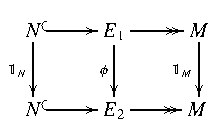
\includegraphics[width=0.46\paperwidth]{figures/Fig_008_PDF041_Book029.pdf}
  \caption{两个等价扩张之间的交换图（原书 p.29）}
  \label{fig:equivalent-extensions}
\end{figure}
\end{definition}

\begin{theorem}{Ext 群分类扩张}{ext-classifies-extensions}
向量空间 $\operatorname{Ext}_A^1(M,N)$ 按等价分类从 $M$ 到 $N$ 的所有扩张。特别地，若 $\operatorname{Ext}_A^1(M,N)=0$，则每个短正合列
\[
  N\lhook\joinrel\longrightarrow E\twoheadrightarrow M
\]
都分裂：$E\cong M\oplus N$。
\end{theorem}
\begin{proof}[证明思路]
给定一个扩张，可以把 $M$ 上的恒等映射沿着分解逐步提升，从而构造一个态射：
\begin{figure}[H]\centering
  \centering
  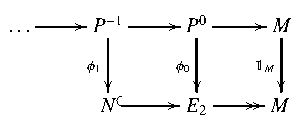
\includegraphics[width=0.40\paperwidth]{figures/Fig_009_PDF042_Book030.pdf}
  \caption{由扩张得到 Ext 群中的元素（原书 p.30）}
  \label{fig:extension-ext-class}
\end{figure}
这会诱导出一个映射类 $[\varphi_1]\in\operatorname{Ext}_A^1(M,N)$。可以证明这个对应是同构；证明见\bookcite{253}的定理 3.4.3。若 $\operatorname{Ext}_A^1(M,N)=0$，则每个扩张都与平凡扩张同构，因而分裂。
\end{proof}

\begin{example}[一个非平凡扩张]\label{ex:nonsplit-extension}
在前面的例子中，可以直接验证短正合列
\[
  \frac{k[X]}{(X-\lambda)}
  \lhook\joinrel\xrightarrow{\ X-\lambda\ }
  \frac{k[X]}{(X-\lambda)^2}
  \twoheadrightarrow
  \frac{k[X]}{(X-\lambda)}
\]
不分裂；它对应于非零 Ext 群中的一个元素。
\end{example}

\subsection{Ext 环}\label{subsec:ext-ring}
给定 $A$-模 $M$ 及其自由分解 $P^\bullet$，Hom 空间 $\operatorname{Hom}_A^\bullet(P^\bullet,P^\bullet)$ 带有由态射复合给出的环结构。由于这一环结构与微分相容，它也在上同调上诱导环结构。因此得到分次环 $\operatorname{Ext}_A^\bullet(M,M)$，并且它不依赖于分解的选择。本节将考察若干特殊情形下 Ext 环的结构。

\begin{example}[对偶数环]\label{ex:dual-numbers-ext}
最简单的情形是 $A=k[X]$、$M=k[X]/(X)$。此时 $M$ 有分解 $F^\bullet=A\xrightarrow{X}A$，并且
\[
  \operatorname{Hom}_A^\bullet(F^\bullet,F^\bullet)=\operatorname{Mat}_2(A),
  \qquad
  df=\begin{pmatrix}0&X\\0&0\end{pmatrix}f
       -(-1)^{\deg f}f\begin{pmatrix}0&X\\0&0\end{pmatrix}.
\]
其同调是二维分次向量空间
\[
  k\begin{pmatrix}1&0\\0&1\end{pmatrix}
  \oplus k\begin{pmatrix}0&1\\0&0\end{pmatrix}
  =:k\iota\oplus k\xi.
\]
生成元 $\xi$ 的次数为 $1$，且 $\xi^2=0$，故
\[
  \operatorname{Ext}_A^\bullet(M,M)\cong\frac{k[\xi]}{\langle\xi^2\rangle}.
\]
这个环称为对偶数环\index{duioushuhuan@对偶数环|hyperpage}。
\end{example}

\begin{example}[平面原点的 Ext 环]\label{ex:ext-polynomial-two-variables}
考察 $A=k[X,Y]$，并令 $S=k[X,Y]/(X,Y)$ 为 $X,Y$ 均平凡作用的简单模。此时有一个很好的分解，称为 Koszul 分解：
\[
  K^\bullet:=A\xrightarrow{\binom{Y}{-X}}A^{\oplus2}
  \xrightarrow{\left(\begin{smallmatrix}X&Y\end{smallmatrix}\right)}A.
\]
结合前面“Ext 群与自由分解的选取无关”这一结论，可知 Ext 群为
\[
  \operatorname{Ext}_A^\bullet(S,S)
  =H\left(S\xrightarrow{\,0\,}S^{\oplus2}\xrightarrow{\,0\,}S\right)
  =k\iota\oplus(k\xi\oplus k\eta)\oplus k\rho,
\]
其中 $\iota,\xi,\eta,\rho$ 依次对应分解中的四个 $A$ 分量，都是把 $a$ 送到 $a\bmod(X,Y)$ 的映射 $A\to S$。我们可以把这四个映射提升为复形态射 $K^\bullet\to K^\bullet$。显然，$\iota$ 提升为恒等映射，而 $\xi,\eta$ 的提升分别如下：
\begin{figure}[H]\centering
  \centering
  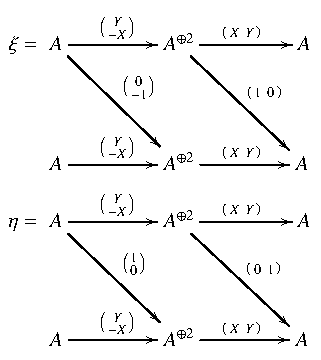
\includegraphics[width=0.70\paperwidth]{figures/Fig_010_PDF043_Book031.pdf}
  \caption{生成元 $\xi$ 与 $\eta$ 的复形态射提升（原书 p.31）}
  \label{fig:ext-generators-lifts}
\end{figure}
这些图不是交换图而是反交换图，因为 $\deg\xi=\deg\eta=1$。它们的复合为
\begin{figure}[H]\centering
  \centering
  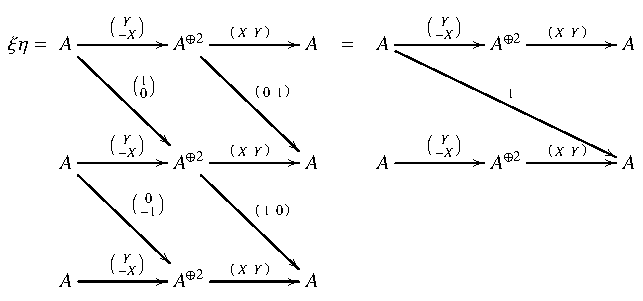
\includegraphics[width=0.70\paperwidth]{figures/Fig_011_PDF043_Book031.pdf}
  \caption{生成元 $\xi$ 与 $\eta$ 的复合（原书 p.31）}
  \label{fig:ext-product-lifts}
\end{figure}
它给出 $\rho$ 的一个提升，而反方向的复合给出 $-\rho$ 的提升。$\xi$ 与自身的复合为零，$\eta$ 与自身的复合也为零。因此
\[
  \operatorname{Ext}_A^\bullet(S,S)
  \cong\frac{k\langle\xi,\eta\rangle}
  {\langle\xi^2,\eta^2,\xi\eta+\eta\xi\rangle}.
\]
% [Tutor Note: $\xi,\eta$ 都是奇次类，而 Ext 环按 Koszul 符号约定分次交换：$\xi\eta=(-1)^{|\xi||\eta|}\eta\xi=-\eta\xi$，所以 $\xi\eta+\eta\xi=0$ 是由次数决定的，与提升的具体取法无关（多项式环情形那条定理中外代数 $\Lambda_n$ 的全部关系都由此而来）。但像“反方向复合给出 $-\rho$ 的提升”“$\xi$ 自乘为零”这类具体结论，仍须把提升按 $K^\bullet$ 的分次逐块相乘、逐块核对符号才能得到，不能只凭分次交换性断言。]
\end{example}

\begin{theorem}{多项式代数的 Ext 环}{polynomial-ext-exterior}
若 $A=k[X_1,\ldots,X_n]$，且 $S=k[X_1,\ldots,X_n]/(X_1,\ldots,X_n)$，则
\[
  \operatorname{Ext}_A^\bullet(S,S)
  \cong
  \frac{k\langle\xi_1,\ldots,\xi_n\rangle}
  {\langle\xi_i\xi_j+\xi_j\xi_i\mid 1\leq i,j\leq n\rangle}
  =:\Lambda_n.
\]
这个代数也称为具有 $n$ 个变量的外代数\index{waidaishu@外代数|hyperpage}\bookcite[第 4.5 节]{253}。
\end{theorem}

我们可以把这一构造推广到更复杂的代数。设代数具有如下形式：
\[
  A=\frac{k\langle X_1,\ldots,X_k\rangle}{\langle r_1,\ldots,r_l\rangle},
\]
其中每个关系都是次数至少为 $2$ 的单项式的线性组合。记 $\langle X_1,\ldots,X_k\rangle$ 为 $X$，记 $\langle r_1,\ldots,r_l\rangle$ 为 $R$，则条件可写作
\[
  R\subset X^2.
\]
此外，假设 $r_i$ 在向量空间 $R/(XR+RX)$ 中构成一组基。若满足此条件，就称 $k\langle X_1,\ldots,X_k\rangle/\langle r_1,\ldots,r_l\rangle$ 是 $A$ 的极小表现\index{jixiaobiaoxian@极小表现|hyperpage}。与多项式环的情形类似，可以考察简单模 $S=A/X$ 及其 Ext 环。

\begin{lemma}{极小表现的自由分解}{minimal-presentation-resolution}
上述模 $S$ 有一个自由分解，其开头部分为
\[
  K^\bullet:=\cdots\longrightarrow A^{\oplus l}
  \xrightarrow{(\partial_i r_j)_{ij}}A^{\oplus k}
  \xrightarrow{(X_1\ \cdots\ X_k)}A,
\]
其中 $\partial_i$ 是一个 $k$-线性算子：若单项式 $X_{s_1}\cdots X_{s_u}$ 的首项为 $X_i$，则
\[
  \partial_i(X_{s_1}\cdots X_{s_u})=X_{s_2}\cdots X_{s_u};
\]
否则结果为零。
\end{lemma}
\begin{proof}[证明思路]
先注意，算子 $\partial_i$ 会从每个关系单项式的首部移除一个 $X_i$，并删去所有无法如此处理的单项式。因此，对每个 $f\in k\langle X_1,\ldots,X_k\rangle$，都有恒等式
\[
  f=\sum_iX_i(\partial_i f).
\]
由于 $X_i$ 是代数 $A$ 的生成元，映射 $A^{\oplus k}\xrightarrow{(X_1\ \cdots\ X_k)}A$ 是满射。现在设 $f_i\in k\langle X_1,\ldots,X_k\rangle$ 满足 $\sum_iX_if_i=r\in R$。可以将 $r$ 写成
\[
  r=\sum_j r_jg_j+u,
\]
其中 $u$ 是形如 $vr_jw$ 的表达式的线性组合，且 $v$ 的次数至少为 $1$。对 $r$ 作用 $\partial_i$，得到
\[
  f_i=\partial_i r=\sum_j(\partial_i r_j)g_j+\partial_i u.
\]
最后一项在 $A$ 中为零，因为 $\partial_i$ 不会作用到关系内部。在 $A$ 中，因而有 $f_i=\sum_j(\partial_i r_j)g_j$，向量 $(f_i)_i$ 是 $(\partial_i r_j)_i$ 的线性组合。因此，分解中的第二个映射覆盖第一个映射的核。其余映射可照常构造：找出 $d_i$ 的核的生成元，再取一个自由模映到这些生成元上。
\end{proof}

这个分解使我们能够描述 Ext 代数的重要一部分及其乘法结构。
\begin{theorem}{Ext 环的低次部分}{ext-low-degrees}
若 $A,S$ 如上，则
\[
  \operatorname{Ext}_A^0(S,S)=k,\qquad
  \operatorname{Ext}_A^1(S,S)=k^{\oplus k}
    =k\xi_1\oplus\cdots\oplus k\xi_k,\qquad
  \operatorname{Ext}_A^2(S,S)=k^{\oplus l}
    =k\rho_1\oplus\cdots\oplus k\rho_l.
\]
并且 $\operatorname{Ext}_A^\bullet(S,S)$ 中的乘积满足如下关系：
\[
  \xi_i\xi_j=\sum_u\lambda^u_{ij}\rho_u
  \quad\Longleftrightarrow\quad
  r_u=\sum_{ij}\lambda^u_{ij}X_jX_i+\text{高次项}.
\]
\end{theorem}
\begin{proof}[证明思路]
将自由分解 $K^\bullet$ 映到 $S$，得到
\[
  S\longrightarrow S^{\oplus k}\longrightarrow S^{\oplus l}
  \longrightarrow\cdots,
\]
其中所有映射均为零。第一个映射为零，是因为生成元在 $S$ 上都作用为零；第二个为零，是因为当 $R\subset\langle X_1,\ldots,X_k\rangle^2$ 时，没有任何 $(\partial_i r_j)$ 含常数项；第三个为零，是因为 $r_i$ 构成 $R/(XR+RX)$ 的一组基。

由于这些映射都为零，
\[
  \operatorname{Ext}_A^1(S,S)=\operatorname{Hom}(A^{\oplus k},S)\cong k^{\oplus k}.
\]
可以选择基元素 $\xi_i$，令它把 $A^{\oplus k}$ 第 $i$ 个直和项中的 $1$ 映到 $1\in S$。这组基与生成元 $X_1,\ldots,X_k$ 对偶。类似地，基 $\rho_1,\ldots,\rho_l$ 属于
\[
  \operatorname{Ext}_A^2(S,S)=\operatorname{Hom}(A^{\oplus l},S)\cong k^{\oplus l},
\]
并与关系 $r_1,\ldots,r_l$ 对偶。结构常数的计算与多项式环情形完全类似。更多细节参见\bookcite{168}。
\end{proof}

\begin{note}
这个定理说明，我们可以从 Ext 环的乘法中恢复关系的二次部分。自然会问：能否进一步恢复三次或更高次部分？单靠乘法做不到；不过上述结果似乎暗示，我们需要定义三重乘积来恢复三次部分、四重乘积来恢复四次部分，依此类推。下一章将看到，确实可以这样做。
\end{note}

\begin{note}
在几何上同调一节中，我们发现环面的上同调环是外代数
\[
  \Lambda_2=\frac{\mathbb C\langle\xi,\eta\rangle}
  {\langle\xi^2,\eta^2,\xi\eta+\eta\xi\rangle};
\]
在代数上同调一节中，我们又发现同一个环可以解释为简单 $\mathbb C[X,Y]$-模的 Ext 环。两个看似无关的对象产生同一个上同调环。这一巧合是构成镜像对称基础的基本事实之一。
\end{note}

\section{练习}\label{sec:cohomology-exercises}
\begin{exercise}\label{exer:cohomology-module-complexes}
引理\ref{lem:complex-map-criterion}对向量空间成立，但推广到更一般的模时，情形会复杂一些。
\begin{enumerate}
  \item 证明引理\ref{lem:complex-map-criterion}对 $\mathbb Z$-模复形不成立。（提示：考察 $\mathbb Z\xrightarrow{2}\mathbb Z$。）
  \item 若 $G$ 是有限群，证明该引理对 $\mathbb C G$-模复形成立。
\end{enumerate}
\end{exercise}

\begin{exercise}\label{exer:simplicial-sets}
单形范畴 $\underline{\Delta}$ 的对象是 $[n]=\{0,\ldots,n\}$，态射是所有非降映射
\[
  \underline{\Delta}([m],[n])=\{\varphi\colon[m]\to[n]\mid x\geq y\Longrightarrow\varphi(x)\geq\varphi(y)\}.
\]
单纯集是从 $\underline{\Delta}$ 到集合范畴的反变函子。注意，严格单调递增单形范畴 $\Delta$ 是 $\underline{\Delta}$ 的子范畴，因此每个单纯集也可以看成一个 $\Delta$-集。反过来，要从 $\Delta$-集得到单纯集，则还需做一些工作。
\begin{enumerate}
  \item 证明若 $S$ 是非平凡单纯集，则对所有 $i\geq0$，$S[i]$ 都非空。
  \item 若 $S$ 是单纯集且 $a\in S[i]$，若 $a$ 属于某个非单射映射 $f$ 下 $S(f)$ 的像，就称 $a$ 为退化单形。令 $S^{\mathrm{nd}}[i]$ 为非退化 $i$-单形所成的集合。证明 $S^{\mathrm{nd}}$ 是一个 $\Delta$-集。
  \item 证明 $C_\Delta^\bullet(S,k)$ 与 $C_\Delta^\bullet(S^{\mathrm{nd}},k)$ 是拟同构复形。
\end{enumerate}
\end{exercise}

\begin{exercise}\label{exer:subdivision}
取一个二维 $\Delta$-集 $S$，并在每个三角形中心增加一个点，将三角形细分如下：
\begin{figure}[H]\centering
  \centering
  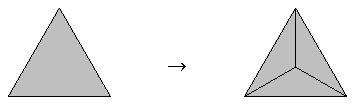
\includegraphics[width=0.40\paperwidth]{figures/Fig_012_PDF046_Book034.pdf}
  \caption{将三角形细分为三个小三角形（原书 p.34）}
  \label{fig:triangle-subdivision}
\end{figure}
证明新的单纯上链复形与原来的上链复形拟同构。
\end{exercise}

\begin{exercise}\label{exer:product-circle}
设 $X=|S|$ 是由 $\Delta$-集 $S$ 给出的拓扑空间，$S^1$ 是圆周。为 $X\times S^1$ 构造一个 $\Delta$-集，并利用它证明
\[
  H^k(X\times S^1,k)\cong H^{k-1}(X,k)\oplus H^k(X,k).
\]
\end{exercise}

\begin{exercise}\label{exer:surface-cohomology}
利用适当的 $\Delta$-集计算亏格为 $g$ 的紧致可定向曲面的上同调环。
\end{exercise}

\begin{exercise}\label{exer:torus-de-rham}
令 $T=\mathbb R^2/\mathbb Z^2$ 为环面，并考察 $\Omega^\bullet(T)$。作为 $C^\infty(T)$-模，它由 $1,dX,dY,dX\wedge dY$ 生成，其中 $X,Y$ 是 $\mathbb R^2$ 上的标准坐标。证明这些元素也构成德拉姆上同调环的一组基。将环面划分为两个三角形，并利用这一划分描述单纯上同调与德拉姆上同调之间的同构。
\end{exercise}

\begin{exercise}\label{exer:surface-group-ext}
考虑环
\[
  R=\frac{\mathbb C\langle X_1,Y_1,\ldots,X_g,Y_g\rangle}
  {\left\langle\sum_i(X_iY_i-Y_iX_i)\right\rangle},
\qquad
  S=R/\langle X_1,Y_1,\ldots,X_g,Y_g\rangle.
\]
计算 $S$ 的 Ext 环。
\end{exercise}

\begin{exercise}\label{exer:truncated-polynomial-ext}
令 $R=\mathbb C[\varepsilon]/(\varepsilon^3)$，$S=R/\langle\varepsilon\rangle$。计算 $S$ 的 Ext 环，并证明在这个环中可以定义一个非零的三元 Massey 积。
\end{exercise}

\begin{exercise}\label{exer:quiver-like-ext}
令
\[
  R=\frac{\mathbb C\langle e,u\rangle}
  {\langle e^2-e,\ eu-u,\ ue\rangle},
\qquad S=R/\langle u\rangle.
\]
证明 $S$ 的 Ext 环同构于 $R$ 本身。
\end{exercise}

\begin{exercise}\label{exer:finite-group-ext}
设 $G$ 是有限群，$V,W$ 是两个 $\mathbb CG$-模。证明当 $i>0$ 时
\[
  \operatorname{Ext}_{\mathbb CG}^i(V,W)=0.
\]
\end{exercise}

\chapterreview{%
\textbf{全章地位。}本章把复形确立为全书的基本工作单位，并把拓扑与代数两条上同调路线并置：一条由 $\Delta$-集通向杯积上同调环，一条由自由分解通向 Ext 环。这是为第 3 章的 $A_\infty$ 结构预备两个“信息不够用”的范例——上同调环丢掉 Massey 积，Ext 环只看得到关系的二次部分。

\textbf{知识脉络。}§2.1 给出上链复形、态射、拟同构与同伦，再用向量空间的分裂 $C^i=H^i\oplus I^i\oplus R^i$ 把拟同构的判定化归为对 $f^{HH}$ 的判定，并得到 $HK^0(k)\simeq\mathrm{grVECT}(k)$。§2.2 用 $\Delta$-集把“粘合空间”翻译成函子，以 $C_\Delta^\bullet(S,k)=\mathrm{Sets}(S[i],k)$ 与杯积建立上同调环，再由奇异上同调与德拉姆定理说明它只依赖 $|S|$。§2.3 把同一句式移植到代数：自由分解、比较定理、Ext 群、扩张的分类、Ext 环与 Koszul 分解。两节末尾各有一个缺口：Massey 积落在环结构之外，乘法又只能恢复二次关系；二者正好汇合，第 3 章由此展开。

\textbf{核心结论。}（1）复形分解为 $C^\bullet\cong C_m^\bullet\oplus C_c^\bullet$，其中 $C_m=H$ 极小、$C_c=I\oplus R$ 可缩，$d$ 在 $R^i\to I^{i+1}$ 上可逆；于是 $f$ 是拟同构当且仅当 $f^{HH}$ 是同构，$f$ 零同伦当且仅当 $f^{HH}=0$。（2）杯积使单纯上同调成为分次环，环面给出 $\Lambda_2=k\langle\xi,\eta\rangle/\langle\xi^2,\eta^2,\xi\eta+\eta\xi\rangle$；若 $|S|\cong X$，则 $HC_\Delta^\bullet(S,k)\cong H^\bullet(X,k)$ 为分次环同构，且 $\varphi\colon\Omega^\bullet(M)\to C_\Delta^\bullet(S,\mathbb R)$ 是拟同构。（3）比较定理保证自由分解间的提升存在且同伦唯一，故 $\operatorname{Ext}_A^i(M,N)$ 与分解的选取无关；$\operatorname{Ext}_A^1$ 按等价分类扩张；对 $A=k[X_1,\ldots,X_n]$ 与 $S=A/(X_1,\ldots,X_n)$，Koszul 分解给出 $\operatorname{Ext}_A^\bullet(S,S)\cong\Lambda_n$。（4）一般地 $\xi_i\xi_j=\sum_u\lambda^u_{ij}\rho_u$ 当且仅当关系 $r_u$ 的二次项为 $\sum_{ij}\lambda^u_{ij}X_jX_i$。

\textbf{辨析与提醒。}其一，“系数在域上”不能省：$\mathbb Z\xrightarrow{2}\mathbb Z$ 说明 $\mathbb Z$-模复形没有 $H\oplus I\oplus R$ 分裂，分解定理与引理\ref{lem:complex-map-criterion} 同时失效，这正是练习 2.1 的要点。其二，两种“上同调相同”并不等同：$|S_1|\cong|S_2|$ 只保证链层面有拟同构，而它一般不是环同构，故拓扑不变性须另证；Massey 积更须在链层面选取 $s,t$。其三，$\langle[u],[v],[w]\rangle$ 是集合而非单个类，符号随 $s,t$ 而变，只有退化为单元素时才“良定义”；第 3 章的 $\mu_3$ 只定到同伦，根源在此。其四，Ext 按上链复形定义，分解写在负次数（$P^0\leftarrow P^{-1}\leftarrow\cdots$），勿与同调次数混同。

\textbf{评注。}本章示范了“同一形式、两种实现”：$\Delta$-集上同调与 Ext 环最终在 $\Lambda_2$ 处重合（§2.3 末注），这就是镜像对称的基本观察。作者刻意只做域系数、只做自由分解，把一般阿贝尔范畴、谱序列与导出函子推给文献；代价是结论偏“玩具”，好处是每个证明都能写成矩阵，读者能亲手看到 $H\oplus I\oplus R$ 与 $h^2=0$、$dhd=d$、$hdh=h$ 这组收缩数据——第 3 章的树形公式正是把它们抽象成沿 $h$ 搬运结构的机器。读本章宜自问：哪些结论真正用到“域”，哪些只用到“复形”？上同调环丢掉的究竟是什么？若只记一个结论，应记住 $f^{HH}$ 这组矩阵分量：它把“拟同构”化为线性代数里的“可逆”。
}
